\addcontentsline{toc}{subsection}{Illustrations: Integration}
\vbtitle{\textbf{Illustrations: Integration}}
\BgThispage
\begin{enumerate}
    \item Find
        \begin{tasks}(2)
            \task $\int_0^1 x^2 \; dx$
            \task $\int_{0}^{\pi/2} \sin^2 x \cdot \cos x \; dx$
            \task $\int_{-1}^1 |x| \; dx$
            \task $\int_0^\pi \sqrt{1 - \sin 2x} \; dx$
            \task $\int_0^3 (|x - 1| + |x - 2|) \; dx$
            \task $\int_{-2}^2 [x] \; dx$
            \task $\int_0^\infty \frac{dx}{1 + x^2}$
            \task $\int_{-1}^2 f(x) \; dx \quad\textit{ where } \quad f(x)= \begin{cases}
                [x] & \textit{if }\quad x \geq 1\\
                0 & \textit{if } \quad 0 \leq x < 1\\
                -x & \textit{if } \quad x < 0
            \end{cases}$
        \end{tasks}
        \vbstarednote{Here, $[x]$ denotes the greatest integer function.}
           \begin{solution}
            \begin{enumerate}
                \item 
                    \begin{align*}
                        \int_0^1 x^2 \; dx &= \left[\frac{x^3}{3}\right]_0^1\\
                        &= \frac{1}{3}
                    \end{align*}

                \item
                    \begin{align*}
                        \int_{0}^{\pi/2} \sin^2 x \cdot \cos x \; dx &= \int_{0}^{\pi/2} \sin^2 x \; d(\sin x)\\
                        \intertext{Let \( u = \sin x \), then \( du = \cos x \; dx \)}
                        \intertext{Limits of \( u \) will be \( 0 \) to \( 1 \) as \( \sin 0 = 0 \) and \( \sin \frac{\pi}{2} = 1 \)}
                        &= \int_{0}^{1} u^2 \; du\\
                        &= \left[\frac{u^3}{3}\right]_0^1\\
                        &= \frac{1}{3}
                    \end{align*}

                \item
                    \begin{align*}
                        &\int_{-1}^1 |x| \; dx\\
                        \intertext{From the definition of the absolute function,}
                        |x| = \begin{cases}
                            x & \text{if } x \geq 0\\
                            -x & \text{if } x < 0
                        \end{cases}
                        \intertext{Apply, $\int_a^b f(x) \; dx = \int_a^c f(x) \; dx + \int_c^b f(x) \; dx$}
                        &= \int_{-1}^0 |x| \; dx + \int_{0}^1 |x| \; dx\\
                        &= \int_{-1}^0 -x \; dx + \int_{0}^1 x \; dx\\
                        &= \left[-\frac{x^2}{2}\right]_{-1}^0 + \left[\frac{x^2}{2}\right]_0^1\\
                        &= \frac{1}{2} + \frac{1}{2}\\
                        &= 1
                    \end{align*}

                \item
                    \begin{align*}
                        \int_0^\pi \sqrt{1 - \sin 2x} \; dx &= \int_0^\pi \sqrt{1 - 2\sin x \cos x} \; dx\\
                        &= \int_0^\pi \sqrt{\sin^2 x + \cos^2 x - 2\sin x \cos x} \; dx\\
                        &= \int_0^\pi \sqrt{(\sin x - \cos x)^2} \; dx\\
                        &= \int_0^\pi |\sin x - \cos x| \; dx\\
                        \because \quad |\sin x - \cos x| &= \begin{cases}
                            \sin x - \cos x & \text{if } \sin x \geq \cos x\\
                            \cos x - \sin x & \text{if } \cos x > \sin x
                        \end{cases}
                    \end{align*}
                    \begin{center}
                        \begin{tikzpicture}
                            \tzaxes(-1.5, -1.5)(5, 1.5){$x$}{$y$}
                            \tzfn{sin(deg(\x))}[0:1.5*pi]
                            \tzfn{cos(deg(\x))}[0:1.5*pi]
                            \tzline(pi/4, 0)(pi/4, 1.2)
                            \tzticks*{0, 0.25*pi, 0.5*pi, 0.75*pi, pi}
                            \tzticks<0, -0.35>{0.25*pi/$\frac{\pi}{4}$, pi/$\pi$}
                        \end{tikzpicture}
                    \end{center}
                    \begin{align*}
                        \intertext{From the graph, as you can see, $\cos x > \sin x$ in $0$ to $\pi/4$ and $\sin x > \cos x$ in $\pi/4$ to $\pi$,}
                        \therefore \quad |\sin x - \cos x| &= \begin{cases}
                            \cos x - \sin x & \text{if } x \in [0, \pi/4]\\
                            \sin x - \cos x & \text{if } x \in [\pi/4, \pi]
                        \end{cases}\\
                        &= \int_0^{\pi/4} (\cos x - \sin x) \; dx + \int_{\pi/4}^\pi (\sin x - \cos x) \; dx\\
                        &= \left[\sin x + \cos x\right]_0^{\pi/4} + \left[-\cos x - \sin x\right]_{\pi/4}^\pi\\
                        &= \left[\sin \frac{\pi}{4} + \cos \frac{\pi}{4} - \sin 0 - \cos 0\right] + \left[-\cos \pi - \sin \pi + \cos \frac{\pi}{4} + \sin \frac{\pi}{4}\right]\\
                        &= \left[\frac{1}{\sqrt{2}} + \frac{1}{\sqrt{2}} - 1 \right] + \left[1 + \frac{1}{\sqrt{2}} + \frac{1}{\sqrt{2}}\right]\\
                        &= 2\sqrt{2}
                    \end{align*}
\BgThispage
                \item
                    \begin{align*}
                        \int_0^3 (|x - 1| + |x - 2|) \; dx &= \int_0^1 (|x - 1| + |x - 2|) \; dx + \int_1^2 (|x - 1| + |x - 2|) \; dx + \int_2^3 (|x - 1| + |x - 2|) \; dx\\
                        &= \int_0^1 (1 - x + 2 - x) \; dx + \int_1^2 (x - 1 + 2 - x) \; dx + \int_2^3 (x - 1 + x - 2) \; dx\\
                        &= \int_0^1 (3 - 2x) \; dx + \int_1^2 (1) \; dx + \int_2^3 (2x - 3) \; dx\\
                        &= \left[3x - x^2\right]_0^1 + \left[x\right]_1^2 + \left[x^2 - 3x\right]_2^3\\
                        &= \left[3 - 1\right] + \left[2 - 1\right] + \left[(9 - 9) -(4-6)\right]\\
                        &= 2 + 1 + 2\\
                        &= 5
                    \end{align*}

                \item
                    \begin{align*}
                        \int_{-2}^2 [x] \; dx &= \int_{-2}^{-1} [x] \; dx + \int_{-1}^{0} [x] \; dx + \int_{0}^{1} [x] \; dx + \int_{1}^{2} [x] \; dx\\
                        \intertext{From the definition of the greatest integer function,}
                        [x] = \begin{cases}
                            -2 & \text{if } x \in [-2, -1)\\
                            -1 & \text{if } x \in [-1, 0)\\
                            0 & \text{if } x \in [0, 1)\\
                            1 & \text{if } x \in [1, 2)
                        \end{cases}\\
                        &= \int_{-2}^{-1} [-2] \; dx + \int_{-1}^{0} [-1] \; dx + \int_{0}^{1} [0] \; dx + \int_{1}^{2} [1] \; dx\\
                        &= \int_{-2}^{-1} -2 \; dx + \int_{-1}^{0} -1 \; dx + \int_{0}^{1} 0 \; dx + \int_{1}^{2} 1 \; dx\\
                        &= \left[-2x\right]_{-2}^{-1} + \left[-x\right]_{-1}^{0} + \left[0\right]_{0}^{1} + \left[x\right]_{1}^{2}\\
                        &= \left[2 - 4\right] + \left[0 + 1\right] + \left[0\right] + \left[2 - 1\right]\\
                        &= 0
                    \end{align*}

                \item
                    \begin{align*}
                        \int_0^\infty \frac{dx}{1 + x^2} \\
                        \intertext{Let \( x = \tan \theta \), then \( dx = \sec^2 \theta \; d\theta \)}
                        \intertext{Limits of \( \theta \) will be \( 0 \) to \( \frac{\pi}{2} \) as \( \tan 0 = 0 \) and \( \tan \frac{\pi}{2} \to \infty \)}
                        &= \int_0^{\pi/2} \frac{\sec^2 \theta \; d\theta}{1 + \tan^2 \theta}\\
                        &= \int_0^{\pi/2} d\theta\\
                        &= \left[\theta\right]_0^{\pi/2}\\
                        &= \frac{\pi}{2}
                    \end{align*}
\BgThispage
                \item
                    \begin{align*}
                        \int_{-1}^2 f(x) \; dx \quad\textit{ where } \quad f(x)= \begin{cases}
                            [x] & \textit{if }\quad x \geq 1\\
                            0 & \textit{if } \quad 0 \leq x < 1\\
                            -x & \textit{if } \quad x < 0
                        \end{cases}
                    \end{align*}
                    \begin{center}
                        \begin{tikzpicture}
                            \tzaxes(-1.5, -1.5)(3.5, 1.5){$x$}{$y$}
                            % \tzline(1, 0)(1, 1)
                            % \tzline(0, 0)(0, -1)
                            \tzfn{\x-\x}[0:1]
                            \tzfn{-\x}[-1:0]
                            \tzfn{1}[1:2]
                            \tzticks*{-1,0, 1, 2}{1}
                            \tzticks<0, -0.35>{-1/$-1$, 1/$1$, 2/$2$}{1}
                        \end{tikzpicture}
                    \end{center}
                    \begin{align*}
                        \int_{-1}^2 f(x) \; dx &= \int_{-1}^0 f(x) \; dx + \int_{0}^1 f(x) \; dx + \int_{1}^2 f(x) \; dx\\
                        &= \int_{-1}^0 -x \; dx + \int_{0}^1 0 \; dx + \int_{1}^2 1 \; dx\\
                        &= \left[-\frac{x^2}{2}\right]_{-1}^0 + \left[0\right]_{0}^1 + \left[x\right]_{1}^2\\
                        &= \left[0 + \frac{1}{2}\right] + \left[0\right] + \left[2 - 1\right]\\
                        &= \frac{1}{2} + 1\\
                        &= \frac{3}{2}
                    \end{align*}
            \end{enumerate}
           \end{solution}



    \item A particle is moving along $x-axis$. Velocity $v_x$ of the particle varies with time $t$ according as \[v_s(t)=t^2-2t-3\]
            Position of the particle at time $t=0$ is $0$ $ie$, $x=0$ at $t=0$. Find the position $x$ of the  particle at time $t=1$. \\
            Velocity $v_x$ is defined as $v_x=\dfrac{dx}{dt}$.
        \begin{solution}
            \begin{align*}
                v_x(t) &= t^2-2t-3\\
                \frac{dx}{dt} &= t^2-2t-3\\
                dx &= (t^2-2t-3)dt\\
                \intertext{Integrating both sides with respect to \( t \), we get}
                \int dx &= \int (t^2-2t-3)dt\\
                x(t) &= \frac{t^3}{3} - t^2 - 3t + C
                \intertext{Given that \( x(0) = 0 \), we can find the value of \( C \) as follows:}
                x(0) &= 0\\
                0 &= \frac{0}{3} - 0 - 0 + C\\
                C &= 0
                \intertext{Therefore, the position of the particle at time \( t = 1 \) is:}
                x(1) &= \frac{1}{3} - 1 - 3\\
                &= -\frac{11}{3}
            \end{align*}
        \end{solution}

        \BgThispage

    \item A force $F_x$ acts on a particle moving along $x-axis$. $F_x$ varies with $x$ according as \[F_x=x^2-x\]
        Find the work done by $F_x$ as the particle moves from $x=0$ to $x=1$.\\[2mm]
        Work done by a force $F_x$ during displacement from $x=x_1$ to $x=x_2$ is defined as $W=\int_{x_1}^{x_2} F_xdx$, where $dx$ is infinitesimal change in the position of the particle.
        \begin{solution}
            \begin{align*}
                F_x &= x^2 - x\\
                \intertext{From the definition of work done,}
                W &= \int_{0}^{1} (x^2 - x)dx\\
                &= \left[\frac{x^3}{3} - \frac{x^2}{2}\right]_{0}^{1}\\
                &= \left[\frac{1}{3} - \frac{1}{2}\right] - \left[0 - 0\right]\\
                &= \frac{1}{3} - \frac{1}{2}\\
                &= -\frac{1}{6}
            \end{align*}
        \end{solution}

        \BgThispage
    \item Velocity $v_x$ of a particle moving along $x-axis$ varies with time $t$ according as \[v_x=t^2-2t+2\]
    A time-varying force $F_x=t+1$ acts on the particle.
    Find the work done by $F_x$ on the particle during time-interval $t=0$ to $t=1$.\\[2mm]
    Work done by a force $F_x$ during displacement from $x=x_1$ to $x=x_2$ is defined as $W=\int_{x_1}^{x_2} F_xdx$, where $dx$ is infinitesimal change in the position of the particle. Velocity $v_x$ is defined as $v_x=\dfrac{dx}{dt}$.
    \begin{solution}
        \begin{align*}
            v_x &= t^2 - 2t + 2\\
            \intertext{From the definition of velocity,}
            \frac{dx}{dt} &= t^2 - 2t + 2\\
            dx &= (t^2 - 2t + 2)dt \tag{1}\\
            \intertext{From the definition of work done and using equation (1),}
            W &= \int_{0}^{1} (t+1)(t^2 - 2t + 2)dt\\
            &= \int_{0}^{1} (t^3 - 2t^2 + 2t + t^2 - 2t + 2)dt\\
            &= \int_{0}^{1} (t^3 - t^2  + 2)dt\\
            &= \left[\frac{t^4}{4} - \frac{t^3}{3} + 2t\right]_{0}^{1}\\
            &= \left[\frac{1}{4} - \frac{1}{3} + 2\right] - \left[0 - 0 + 0 + 0\right]\\
            &= \frac{1}{4} - \frac{1}{3} + 2\\
            &= \frac{23}{12}
        \end{align*}
    \end{solution}

\BgThispage
    \item Velocity $v_x$ of a particle moving along $x-axis$ varies with time $t$ according as \[v_x=t^2-2\]
    A time-varying force $F_x=2t$ acts on the particle.
    Find the power delivered by $F_x$ the force $F_x$ to the particle as a function of time $t$.\\[2mm]
    Power $P$ is defined as $P=\dfrac{dW}{dt}$, where \[W=\int F_x dx \qquad \text{and} \qquad v_x=\dfrac{dx}{dt}\]
    \begin{solution}
        \begin{align*}
            v_x &= t^2 - 2\\
            \intertext{From the definition of velocity,}
            \frac{dx}{dt} &= t^2 - 2\\
            dx &= (t^2 - 2)dt \tag{1}\\
            \intertext{From the definition of work done and using equation (1),}
            W &= \int (2t)(t^2 - 2)dt\\
            &= \int (2t^3 - 4t)dt\\
            &= \left[\frac{2t^4}{4} - \frac{4t^2}{2}\right]\\
            &= \frac{t^4}{2} - 2t^2 + C
            \intertext{From the definition of power,}
            P &= \frac{dW}{dt}\\
            &= \frac{d}{dt}\left(\frac{t^4}{2} - 2t^2 + C\right)\\
            &= \frac{4t^3}{2} - 4t\\
            &= 2t^3 - 4t
        \end{align*}    
    \end{solution}
    \BgThispage
\end{enumerate}